%% Latex Template for 16-720J student reports
%% You should maintain the template format wherever practical
%% Gary Overett 2015

\documentclass[12pt]{article}
\usepackage{amsmath}
\usepackage{amssymb}
\usepackage{amsthm}
\usepackage{amscd}
\usepackage{amsfonts}
\usepackage{graphicx}
\usepackage{subcaption}
\usepackage{fancyhdr}
\usepackage{tablefootnote}
\usepackage{subcaption}
\usepackage[table]{xcolor}
\usepackage{array,multirow}
\usepackage{hyperref}
\usepackage{enumerate}
\usepackage{titling}
\usepackage{titlesec}
\usepackage{float}
\usepackage[a4paper, margin=2cm]{geometry}
\usepackage[framed,numbered,autolinebreaks,useliterate]{mcode}

\titleformat{\subsubsection}{\bf}{Question \arabic{section}.\arabic{subsection}.\arabic{subsubsection} }{0pt}{}[]

%% \topmargin-2cm
%% \textheight+23cm

%% \textwidth6.5in

%% \setlength{\topmargin}{0in} \addtolength{\topmargin}{-\headheight}
%% \addtolength{\topmargin}{-\headsep}

%% \setlength{\oddsidemargin}{0in}

%% \oddsidemargin  0.0in \evensidemargin 0.0in 

\newcounter{list}

\setlength{\droptitle}{-2cm} % less room above the title

\begin{document}

\title{16720J: Homework 3 - Object Detection}

\author{Wenbo Zhao\\
(wzhao1@andrew.cmu.edu, NetID: zhaowb7)}
\date{October 25, 2015}

\maketitle

\emph{{\bf Collaboration declaration}: This homework is done in partial collaboration with Wenbo Liu() and Yan Xu(). Specifically, for Q.~\ref{exemplars}, the author discussed the methods of finding nearest examplars to cluster centers with them and adopted the one with counting pixel label membership. The author also discussed with them on selecting new features for clustering. The author thanks them for their contribution to this work.}

\section{Warming up with some theory (9pts)}

\renewcommand{\thesubsection}{\bf Question \arabic{section}.\arabic{subsection}}

\subsection{(2pts, 1 line)}
$(M-h+1)\times(N-w+1)$ windows.

\subsection{(5pts, 2-3 lines)}
Algorithms that optimize the area under the ROC curve are not guaranteed to optimize the area under the PR curve \cite{Davis:2006:RPR:1143844.1143874}. E.g. if the number of negative examples outnumbers positive examples, ROC curve can't capture the effect of large number change of false positives, since it leads to small variation in false positive rate, while precision captures this change.
\subsection{(2 pts, 1 line)}
1000. 1. 

\section{Object Detection via DPMs and Non-Maximum Suppression (40 pts)}
\label{dpm}

\renewcommand{\thesubsection}{\arabic{section}.\arabic{subsection}}

\subsection{Mean-Shift Clustering (20 pts)}

\subsubsection{\texttt{MeanShift.m}}

\lstinputlisting{../HW3-release/code/baselineDPM/MeanShift.m}

\subsubsection{}

Save your \texttt{CCenters} and \texttt{CMemberships} into \texttt{q21\_result.mat}.
Also save the visualization result from \texttt{q21\_test.m}, as \texttt{q21\_clustering.jpg} and include here.

\begin{figure}[H]
  \centering 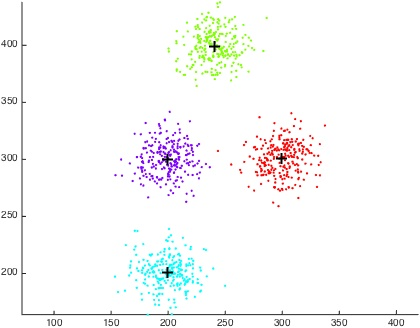
\includegraphics[width=0.6\linewidth]{../HW3-release/code/baselineDPM/q21_clustering.jpg}
  \caption{Mean Shift Clusters}
  \label{clusters}
\end{figure}

\lstinputlisting{../HW3-release/code/baselineDPM/q21_test.m}
\subsubsection{(at most 3 lines in your write-up)}
\label{q:bandwidth}
For low bandwidth, too many number of clusters are found, this is not reasonable when a group of points have large inter-cluster distance but slightly large in-cluster distance and would fall into different clusters. So tune up the bandwidth until the cluster is reasonably placed.

\subsection{Detecting using Deformable Part Models (DPMs) (20 pts)}

\subsubsection{}

Submit your \texttt{nms} function and include here

\lstinputlisting{../HW3-release/code/baselineDPM/nms.m}

\subsubsection{(at most 3 lines in your write-up)}
Given input detection boxes, what nms does is treating the boxes as feature points and cluster them. So picking top-K candidates is equivalent to, as in Q.~\ref{q:bandwidth}, tuning bandwidth, and K is not necessarily to be significantly vary -- they basically yield the same cluster numbers.

\subsubsection{}

Your result images here:

\begin{figure}[H]
  \centering
  \begin{minipage}[t]{0.45\textwidth}
  \centering
  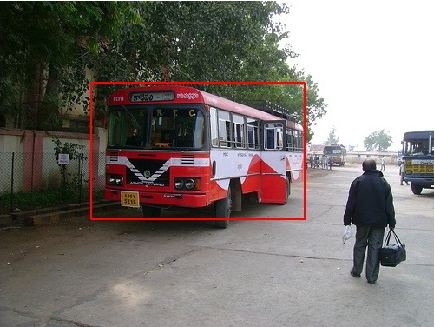
\includegraphics[width=\linewidth]{../HW3-release/code/baselineDPM/q22_result}
  % \centerline{(a) NMS Result 1}
  \caption*{(a) NMS Result 1 }
  \end{minipage}
\hfill
  \begin{minipage}[t]{.45\textwidth}
  \centering
  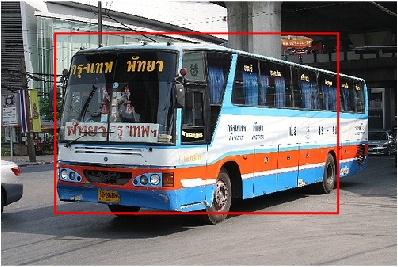
\includegraphics[width=\linewidth]{../HW3-release/code/baselineDPM/q22_result1}
  \caption*{(b) NMS Result 2}
  \end{minipage}
\vfill
  \begin{minipage}[t]{.45\textwidth}
  \centering
  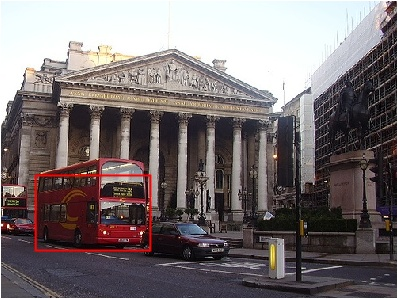
\includegraphics[width=\linewidth]{../HW3-release/code/baselineDPM/q22_result2}
  \caption*{(c)NMS Result 3}
  \end{minipage}
\hfill
  \begin{minipage}[t]{.45\textwidth}
  \centering
  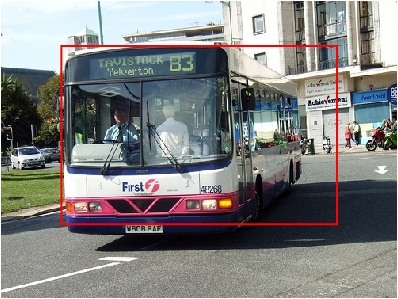
\includegraphics[width=\linewidth]{../HW3-release/code/baselineDPM/q22_result3}
  \caption*{(d)NMS Result 4}
  \end{minipage}
\vfill
  \begin{minipage}[t]{.45\textwidth}
  \centering
  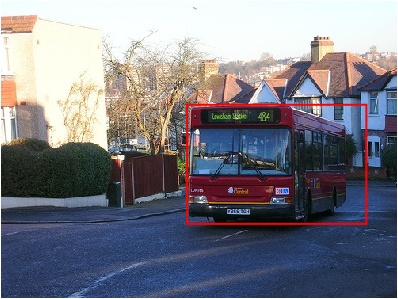
\includegraphics[width=\linewidth]{../HW3-release/code/baselineDPM/q22_result4}
  \caption*{(e)NMS Result 5}
  \end{minipage}
\hfill
  \begin{minipage}[t]{.45\textwidth}
  \centering
  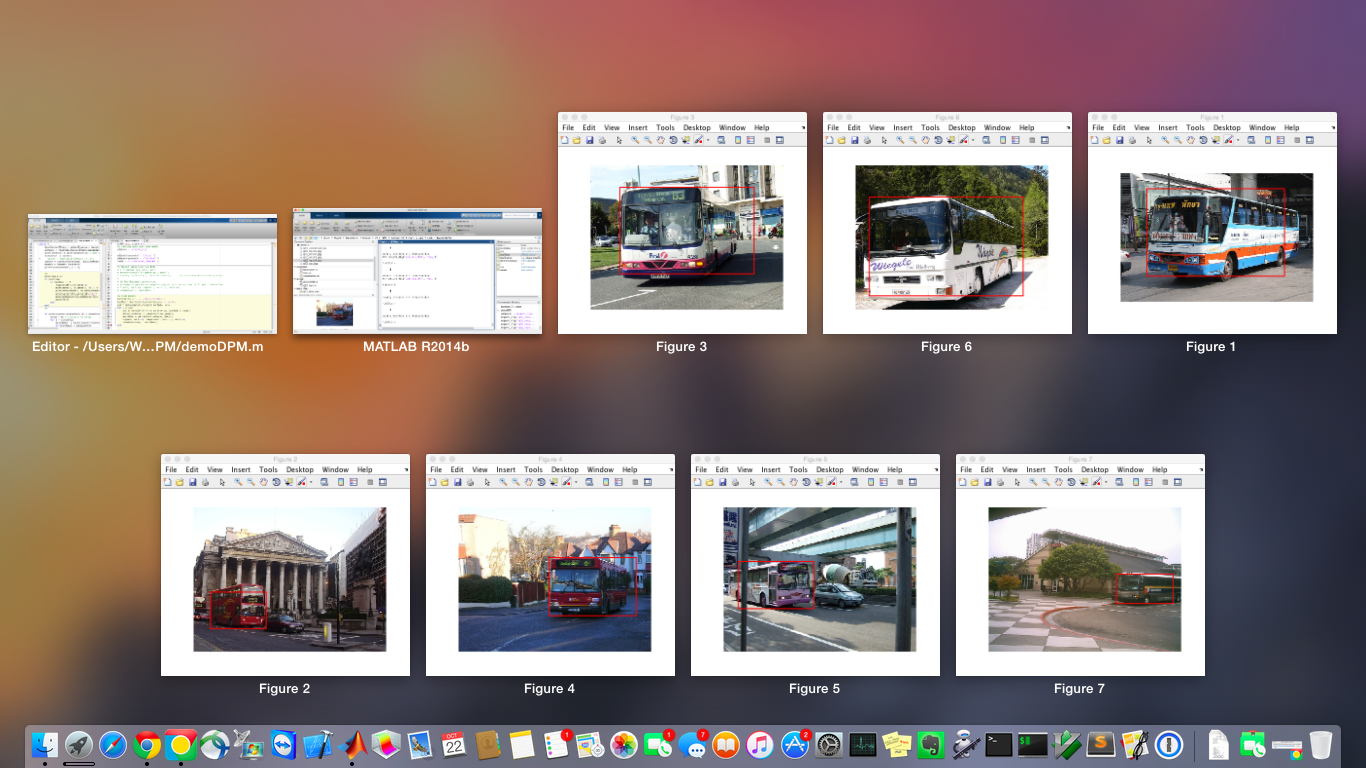
\includegraphics[width=\linewidth]{../HW3-release/code/baselineDPM/q22_result5}
  \caption*{(f)NMS Result 6}
  \end{minipage}

\caption{NMS results}
\label{fig:nms_results}
\end{figure}

\lstinputlisting{../HW3-release/code/baselineDPM/demoDPM.m}

\section{Reducing Exemplar Detectors (55 pts)}
\label{exemplars}

\subsection{Detecting using Exemplar Detectors (10 pts)}

\subsubsection{(10 pts)}

\lstinputlisting{../HW3-release/code/baselineESVM/batchDetectImageESVM.m}

\subsection{Evaluating Detection Performance (15 pts)}

\subsubsection{Theory (5 pts, 2 lines)}

Average precision (AP) is the average value of precision over recall $p(r)$ in the precision-recall curve, and is calculated by $AP = \int_0^1 p(r)dr$.

\subsubsection{(10 pts)}

Submit your script as \texttt{q3\_2\_2.m} and include here. Include an interpretation of your graph here.

\begin{figure}[H]
  \centering 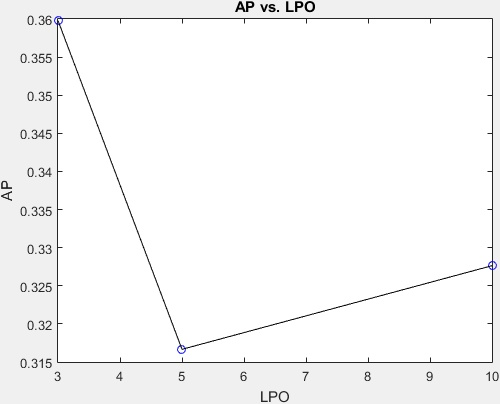
\includegraphics[width=0.6\linewidth]{../HW3-release/code/baselineESVM/AP_LPO.jpg}
  \caption{{\bf AP vs LPO (test set)} A higher
lpo implies more levels in the HOG feature pyramid. It shows that with 3 layers we get the best AP result, and as the layers increase, the AP value decreases might due to too many layers of scaling.}
  \label{clusters}
\end{figure}

\lstinputlisting{../HW3-release/code/baselineESVM/q3_2_2.m}

\subsection{Compacting the set of exemplar detectors}

\subsubsection{(20 pts)}
\label{filtbank}

\begin{figure}[H]
  \centering 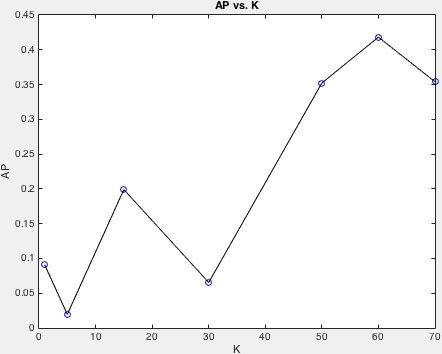
\includegraphics[width=0.6\linewidth]{../HW3-release/code/baselineESVM/AP_vs_K.jpg}
  \caption{{\bf K vs AP} \\ 
  {\it NOTE: AP values vary each run}}
  \label{fig:k_vs_ap}
\end{figure}

\begin{figure}[H]
  \centering 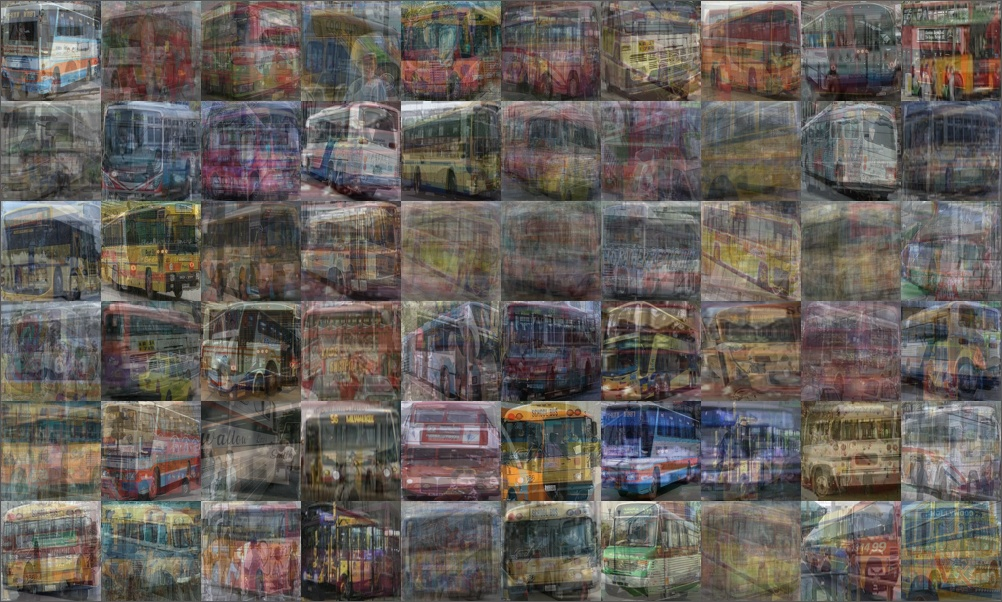
\includegraphics[width=0.6\linewidth]{../HW3-release/code/baselineESVM/average_img_k=60.jpg}
  \caption{Average Images (K=60)}
  \label{fig:ave_img_k60}
\end{figure}

\lstinputlisting{../HW3-release/code/baselineESVM/q3_3_1.m}

\subsubsection{(10 pts)}

In this section different features
\begin{enumerate}[(a)]
\item HOG
\item SIFT
\item dense SIFT (too slow on running, give up... see code below)
\end{enumerate}
are tried. Results are shown below.

\begin{figure}[H]
  \centering \includegraphics[width=0.6\linewidth]{../HW3-release/code/baselineESVM/hog_AP_vs_K.jpg}
  \caption{K vs AP (HOG feature)}
\end{figure}

\begin{figure}[H]
  \centering \includegraphics[width=0.6\linewidth]{../HW3-release/code/baselineESVM/hog_average_img_k=60.jpg}
  \caption{Average Images (HOG feature, K=60)}
\end{figure}

\begin{figure}[H]
  \centering \includegraphics[width=0.6\linewidth]{../HW3-release/code/baselineESVM/sift_AP_vs_K.jpg}
  \caption{K vs AP (SIFT feature)}
\end{figure}

\begin{figure}[H]
  \centering \includegraphics[width=0.6\linewidth]{../HW3-release/code/baselineESVM/sift_average_img_k=60.jpg}
  \caption{Average Images (SIFT feature, K=60)}
\end{figure}

\lstinputlisting{../HW3-release/code/baselineESVM/q3_3_2.m}

\section{Extra credit: Segmentation transfer using ESVM (20 pts)}

If you have attempted this extra-credit section please include a summary of your efforts here and include all relevant
work in the folder \texttt{segTransfer}.\\
\\
\textbf{Thoughts}: The basis concept is replacing the detected bounding boxes of targets (using HOG features and E-SVM detectors) with the corresponding masks, either the masks be meta-data or segmentation superpixels. Specifically, one can first train the E-SVM detector with examplar HOG features, and then detect targets on the test set. For the detected targets, they correspond to a pre-defined meta-data (or segmentation superpixels). What we need to do is aligning this meta-data to the detected bounding boxes (resizing the meta-data to the box size). 

\bibliographystyle{ieeetr} 
\bibliography{hw3.bib}

\end{document}
